Pour pouvoir transmettre les messages depuis l'utilisateur vers le téléphone portable, nous avons
choisi de mettre en place un site web à l'allure d'un gestionnaire de conversation. 
blablabla

Le fonctionnement de ce projet repose grandement sur la partie qui suit.
\\



%%%%%%%%%%%%%%%%%%%%%%%%%%%%%%%%%%%%%%%%%%%%%%%%%%%%%%%%%%%%%%%%%%%%%%%%%%%%%%%%%%%%%%%%%%%%%%%%%%%%
\subsection{Play Framework 2.0}
%%%%%%%%%%%%%%%%%%%%%%%%%%%%%%%%%%%%%%%%%%%%%%%%%%%%%%%%%%%%%%%%%%%%%%%%%%%%%%%%%%%%%%%%%%%%%%%%%%%%

\subsubsection{Primefaces vs Play Framework}

Pour créer notre webservice, nous souhaitions utiliser des technologies récentes. Nous nous sommes
alors confrontés à deux choix complètement opposés. Premièrement, utilisé le jeune Play Framework 
qui est un framework d'application web RESTFul. Le deuxième candidat, Primefaces, est un framework
basé sur les JSF. Il contient une bibliothèque graphique très riche.

Notre choix s'est porté sur Play dont l'approche original nous à attirer. Play Framework est basé sur
les langages Java et Scala et permet le développement sur ces deux langages. C'est un framework RESTFul
ce qui implique que le serveur ne gère pas d'état pour les clients.
\\


%%%%%%%%%%%%%%%%%%%%%%%%%%%%%%%%%%%%%%%%%%%%%%%%%%%%%%%%%%%%%%%%%%%%%%%%%%%%%%%%%%%%%%%%%%%%%%%%%%%%
\subsection{Authentification avec OAuth 2.0} % voir si l'on ne peut pas factoriser du rapport avec la partie Androïd
%%%%%%%%%%%%%%%%%%%%%%%%%%%%%%%%%%%%%%%%%%%%%%%%%%%%%%%%%%%%%%%%%%%%%%%%%%%%%%%%%%%%%%%%%%%%%%%%%%%%

L'authentification des utilisateurs est un point sensible lors du développement d'un service car il
implique souvent le stockage des mots de passes et donc de sécuriser l'application, veiller à corriger
les failles de sécurité,... 

Le protocole OAuth 2.0 permet de contourner ce problème en délégant la gestion de l'authentification
à une autre entité. Beaucoup de services internet populaire implémentent ce système ce qui permet de 
aux utilisateurs de se connecter à un service en utilisant un de leurs comptes déjà existant. Ce 
protocole facilite donc la connexion pour le service qui l'utilise et les utilisateurs qui n'ont pas 
à créer un nouveau compte sur chaque nouveau site web par exemple.

Nous avons alors décider d'utiliser OAuth 2.0 car nous ne souhaitions pas d'une part mettre en place 
et administrer une base de donnée et d'autre part, nous ne voulions pas avoir à gérer la sécurité de 
des données stockés. OAuth s'est donc avéré comme la solution idéale pour notre projet.
\\

\paragraph{Fonctionnement -}

Comme le montre le schéma \ref{schema-oauth-google}, l'authentification se compose de plusieurs étapes.
Premièrement, l'utilisateur va se voir rediriger vers les sites de Google ou il devra donner son accord
à l'application d'effectuer des actions sur son compte. Dans notre cas, il s'agissait comme le montre
l'impression d'écran \ref{croquette-droit-delegation} de pouvoir récupérer les contacts et d'utiliser 
le compte GTalk de l'utilisateur.

Une fois que l'utilisateur à accepter, il doit s'identifier sur la plateforme de Google avec ses identifiants.
Si l'authentification réussi alors l'application se voit offrir un token. Elle doit alors échanger 
son token avec les serveurs de google dans le but d'obtenir un token d'accès. Si tout se déroule correctement,
elle obtient le token d'accès.

Lors de chaque requête pour récupérer des informations sur l'utilisateur, le webservice devra alors
joindre son token d'accès à la requête pour avoir une réponse. De cette manière, nous pouvons récupérer
des informations de l'utilisateur sans utiliser son mot de passe et son identifiant. Nous déléguons donc
la sécurisation du mot de passe à Google.

Nous avons choisi d'utiliser l'authentification avec la plateforme Google car nous pouvions ainsi 
successivement, s'authentifier sur GTalk et récupérer les contacts de l'utilisateur.
\\



%%%%%%%%%%%%%%%%%%%%%%%%%%%%%%%%%%%%%%%%%%%%%%%%%%%%%%%%%%%%%%%%%%%%%%%%%%%%%%%%%%%%%%%%%%%%%%%%%%%%
\subsection{Gestion des contacts}
%%%%%%%%%%%%%%%%%%%%%%%%%%%%%%%%%%%%%%%%%%%%%%%%%%%%%%%%%%%%%%%%%%%%%%%%%%%%%%%%%%%%%%%%%%%%%%%%%%%%

La gestion des contacts de l'utilisateur est un point important de notre projet.
De plus notre cahier des charges spécifie leurs gestion simple et transparente.
\\


\subsubsection{Téléchargement des contacts Google}
\label{Téléchargement des contacts Google}

Par défaut sous Androïd les contacts du téléphone sont dupliqués sur le serveur Google grâce au compte associés au smartphone, ce qui permet d'avoir une synchronisation sur tous les services Google dont Gmail.
\\


Étant connecté sur notre site internet via son compte Google, notre application web va ainsi pouvoir récupérer la liste des contacts de l'utilisateur grâce au token délivré par Google lors de l'authentification.
\\

%%%%%%%%%%%%%%%%%%%%%%%%%%%%%%%%%%%%%%%%%%%%%%%%%%%%%%%%%%%%%%%%%%%%%%%%%%%%%%%%%%%%%%%%%%%%%%%%%%%%

\subsubsection{Tri et Formatage}

Le carnet de contacts de l'utilisateur peut contenir de nombreux types de numéros : téléphone mobiles, téléphone fixes, numéros étrangers, numéros surtaxés, ...
Nous avons donc filtré la liste des contacts aux numéros de mobiles, c'est-à-dire ceux commençant par "0" ou "+33" suivi de 9 chiffres.

Cela permet de ne pas surcharger la liste des contacts avec de nombreux numéros à qui l'on envoie jamais de SMS.
De plus c'est un aspect sécuritaire car l'utilisateur ne pourra pas envoyer des SMS surtaxés depuis le site web.
\\

%%%%%%%%%%%%%%%%%%%%%%%%%%%%%%%%%%%%%%%%%%%%%%%%%%%%%%%%%%%%%%%%%%%%%%%%%%%%%%%%%%%%%%%%%%%%%%%%%%%%

\subsubsection{Google Guava}

Une fois la liste des contacts téléchargés il est nécessaire de la stocker.
Il existe plusieurs types de stockages.

Une \textit{base de données} permet de stocker efficacement des données.
Nous avons voulu proposer aux utilisateurs une solution "sûre" dans laquelle aucune donnée ne sera enregistrées sur le serveur, ce qui implique que l'on n'utilisera pas cette méthode.

La \textit{session} est une courte période pendant laquelle le serveur web communique avec le client (l'utilisateur).
Durant cette période une quantité de mémoire est allouée au client pour y stocker différentes informations, que l'on appelle "variable de session".
Dans Play la notion de "session" est quasiment inexistante en raison de sa nature "RESTful", c'est à dire qui ne conserve pas de données liées aux clients durant la session.

Play propose l'utilisation de \textit{caches} qui est une zone mémoire commune à toutes les utilisateurs, mais avec une durée de vie limitée.
Lorsque le délai est écoulé les données sont effacées automatiquement.
Le problème de cette solution sont les nombreux tests à effectuer pour vérifier que les données sont toujours présentes et effectuer la mise à jour à chaque fois que le cache est vidé.

Nous avons utilisé la classe \lstinline{CacheBuilder} de la bibliothèque Java \textit{Guava} proposé par Google.
Cette classe agit globalement comme un cache (association clé-valeur, durée de vie limitée) tout en ajoutant de nombreuses fonctionnalités.
Il est notamment possible de définir une fonction qui sera exécutée lors de chaque "mise à jour" du cache, qui dans notre cas rafraichira la liste des contacts de l'utilisateur.
\\



%%%%%%%%%%%%%%%%%%%%%%%%%%%%%%%%%%%%%%%%%%%%%%%%%%%%%%%%%%%%%%%%%%%%%%%%%%%%%%%%%%%%%%%%%%%%%%%%%%%%
\subsection{Envoi des messages avec les websockets}
%%%%%%%%%%%%%%%%%%%%%%%%%%%%%%%%%%%%%%%%%%%%%%%%%%%%%%%%%%%%%%%%%%%%%%%%%%%%%%%%%%%%%%%%%%%%%%%%%%%%



\subsubsection{Websocket}



\subsubsection{Notifications}

Lors de la réception d'un SMS l'application mobile va envoyer un message XMPP qui sera reçu par le serveur web.
Le serveur va ensuite envoyer une notification à l'utilisateur grâce à la websocket qui sera traitée en JavaScript dans le navigateur web de l'utilisateur.
Cette notification consiste à indiquer le nombre de messages non lus pour un contact.
Lorsque l'utilisateur affiche la conversation la notification éventuelle est effacée.
Le schéma \ref{siteWeb_notifications} montre un exemple de notification.
\begin{figure}[!h]
	\center
	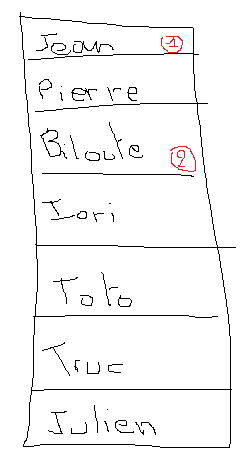
\includegraphics[width=0.3\textwidth]{img/siteWeb_notifications.png}
	\caption{Site web : notifications}
	\label{siteWeb_notifications}
~~\\
\end{figure}


%%%%%%%%%%%%%%%%%%%%%%%%%%%%%%%%%%%%%%%%%%%%%%%%%%%%%%%%%%%%%%%%%%%%%%%%%%%%%%%%%%%%%%%%%%%%%%%%%%%%
\subsection{Design du site}
%%%%%%%%%%%%%%%%%%%%%%%%%%%%%%%%%%%%%%%%%%%%%%%%%%%%%%%%%%%%%%%%%%%%%%%%%%%%%%%%%%%%%%%%%%%%%%%%%%%%

Le design du site est l'un des thèmes que nous avons travaillé pour cette partie la du projet.

Nous souhaitions initialement avoir une interface simple, sans fioritures car cela nous semblait comme
secondaire. Nous avons donc utilisé deux frameworks pour nous faciliter la tache et accélérer la mise
en place du design.

Nous avons donc tout d'abord choisi "Twitter Bootstrap" puis nous l'avons couplé au framework "jQuery
Layout".
\\


\subsubsection{Twitter Bootstrap}

\textit{Twitter Bootstrap}\footnote{Site web : \href{http://twitter.github.com/bootstrap/}{http://twitter.github.com/bootstrap/}} est un framework web utilisé pour le développement front end.
C'est un outil écrit en JavaScript et CSS qui permet de réaliser facilement des interfaces élégantes néanmoins simples. 

Il nous a été utile principalement pour pouvoir concevoir l'affichage des zones d'entrée de textes ou 
encore pour organiser l'affichage des contacts proprement.
\\


\subsubsection{jQuery Layout}

\textit{jQuery Layout}\footnote{Site web : \href{http://layout.jquery-dev.net/}{http://layout.jquery-dev.net/}} est aussi un framework web qui, contrairement à Twitter Bootstrap, permet d'organiser les sites en plusieurs interfaces distinctes. 
L'utilité de JQuery Layout réside dans sa possibilité à fractionner un espace en plusieurs fenêtres.
Cela permet de retrouver l'ergonomie et le coté simple et ordonné des logiciels. 

Ce framework très riche nous a donc été très profitable pour pouvoir obtenir une bonne ergonomie sans avoir
à trop passer du temps sur cette partie.
Le schéma \ref{siteWeb_jQueryLayout} représente l'agencement général de notre site web grâce à ce framework.

\begin{figure}[!h]
	\center
	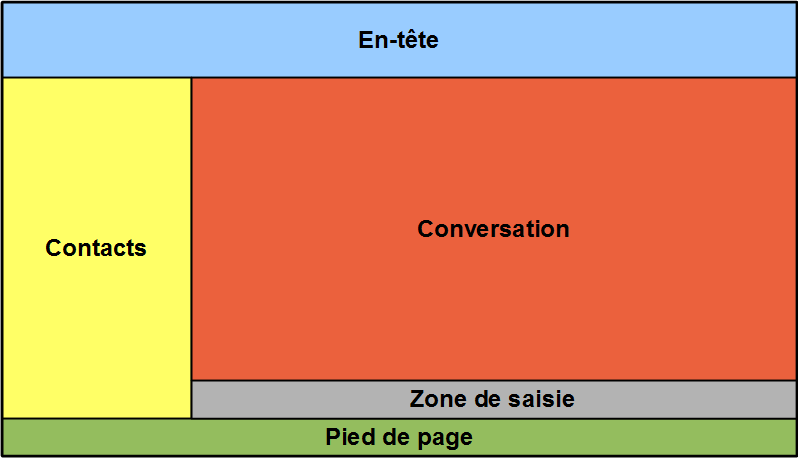
\includegraphics[width=0.6\textwidth]{img/siteWeb_jQueryLayout.png}
	\caption{jQuery Layout : structure du site web}
	\label{siteWeb_jQueryLayout}
~~\\
\end{figure}
